% All Units Milestones Review — running header from here onward
\runningheader{Mathematics 6}{All Units Milestones Review}{Page \thepage\ of \numpages}

\begingradingrange{allmilestones}

\subsection*{All Units Milestones Review}

\question[5]
Nicole has $16$ dolls in her room. Her sister, Amy, has $\dfrac{5}{8}$ of Nicole's dolls in her room. How many dolls does Amy have in her room?
\rightfillin{$10$}
\begin{solution}
  $\dfrac{5}{8}\cdot 16 = 10$.
\end{solution}

\question[5]
Determine which measure of central tendency is most appropriate for the following data and why. Prices for video game consoles: $\$200$, $\$225$, $\$250$, $\$275$, $\$295$, $\$575$.
\begin{choices}
  \choice Mean, since the mean gets the average from the data.
  \choice Median, since the middle number gives the average price.
  \choice Mode, since there will be no outliers in the data.
  \CorrectChoice Median, since there is an outlier that may significantly affect the mean.
\end{choices}
\begin{solution}
  $\$575$ is an outlier; the median is more representative than the mean.
\end{solution}

\question[10]
Find the mean, median, and mode for this data set: $72$, $80$, $80$, $84$, $90$, $92$, $92$, $92$.
\labeledfillin{Mean}{$\dfrac{165}{2}$ (or $82.5$)}
\labeledfillin{Median}{$87$}
\labeledfillin{Mode}{$92$}
\begin{solution}
  Mean $=\dfrac{660}{8}=82.5$; ordered data give median $\dfrac{84+90}{2}=87$; mode $=92$.
\end{solution}

\question[10]
The display shows meal prices (in dollars). Which of the following statements are true? List every true statement by letter (\textbf{A}--\textbf{D}). For \textbf{Range} and \textbf{IQR}, give numeric values from the display.
\begin{center}
  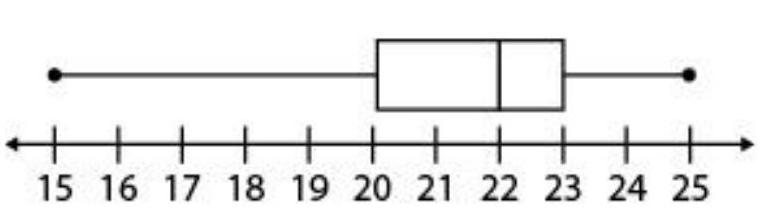
\includegraphics[width=0.88\linewidth]{math-6th/images/25b2bbb6-511f-4540-805d-d84ad3778da8-1_214_766_1353_1250}
\end{center}
\begin{center}
  \textbf{Meal Prices (\$)}
\end{center}
\begin{quote}
  \textbf{A.}\ The median number is $22$.\\
  \textbf{B.}\ The range is $3$.\\
  \textbf{C.}\ The interquartile range is $10$.\\
  \textbf{D.}\ Half of the meal prices are $\$22$ or higher.
\end{quote}
\labeledfillin{True statements (letters)}{}
\labeledfillin{Range}{}
\labeledfillin{Interquartile range}{}
\begin{solutionorbox}[0.75in]
  Read the five-number summary from the plot and test each statement. Range is largest minus smallest price; IQR is third quartile minus first quartile.
\end{solutionorbox}

\question[5]
Order the following from least to greatest:
\[
  8.4,\quad |-4|,\quad 8\frac{3}{8},\quad |9|,\quad -7,\quad -12,\quad \frac{5}{9}\text{.}
\]
\rightfillin[3.2in]{$-12,\ -7,\ \dfrac{5}{9},\ 4,\ 8\frac{3}{8},\ 8.4,\ 9$}
\begin{solution}
  Values: $-12$, $-7$, $\frac{5}{9}$, $4$, $8.375$, $8.4$, $9$.
\end{solution}

\question[5]
Mandy spent $\$72$ on $24$ gallons of gas. At this rate, how many gallons of gas would she have if she spent $\$60$ on gas?
\rightfillin{$20$}
\begin{solution}
  $\dfrac{72}{24}=3$ dollars per gallon; $\dfrac{60}{3}=20$ gallons.
\end{solution}

\question[5]
The height above the ground of a person riding an escalator is shown in the table. What is the missing value in the table?
\begin{center}
  \small
  \begin{tabular}{|l|l|}
    \hline
    Time since getting on escalator & Height above the ground \\
    \hline
    $2$ seconds & $18$ inches \\
    \hline
    $5$ seconds & $45$ inches \\
    \hline
    $7$ seconds & $?$ \\
    \hline
    $10$ seconds & $90$ inches \\
    \hline
    $14$ seconds & $126$ inches \\
    \hline
  \end{tabular}
\end{center}
\begin{choices}
  \choice $54$ inches
  \choice $60$ inches
  \CorrectChoice $63$ inches
  \choice $72$ inches
\end{choices}
\begin{solution}
  Height increases $9$ inches per second; at $7$ s: $18+9(7-2)=63$ inches.
\end{solution}

\question[5]
Rylie has $8$ highlighters, $6$ pens, and $10$ pencils in her pencil pouch. What is the ratio of pencils to the total number of utensils in her bag? Write your answer in simplest form.
\rightfillin{$\dfrac{5}{12}$}
\begin{solution}
  $\dfrac{10}{8+6+10}=\dfrac{10}{24}=\dfrac{5}{12}$.
\end{solution}

\newpage

\question[10]
The school drama club practiced their play in the gym. The director marked off the gym floor in two sections: the stage is in the shape of a trapezoid, and the audience area is in the shape of a rectangle. The diagram of the floor is shown below. What is the total area of both sections?
\begin{center}
  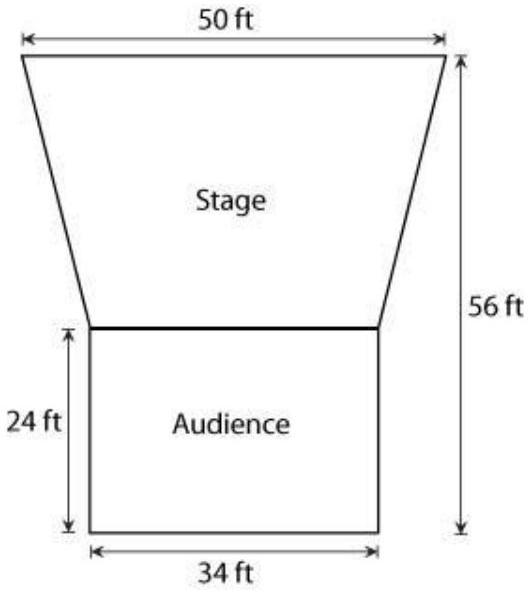
\includegraphics[width=0.88\linewidth]{math-6th/images/25b2bbb6-511f-4540-805d-d84ad3778da8-2_592_532_459_1400}
\end{center}
\begin{solutionorbox}[1.5in]
  Compute the rectangle area and the trapezoid area from the labeled dimensions and add.
\end{solutionorbox}

\question[10]
For an art project, Krista is painting the outside of a cardboard box represented by this net. What is the total area that she needs to paint?
\begin{center}
  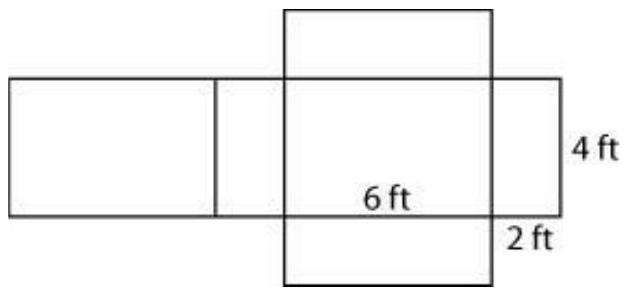
\includegraphics[width=0.88\linewidth]{math-6th/images/25b2bbb6-511f-4540-805d-d84ad3778da8-2_293_626_1095_1226}
\end{center}
\begin{solutionorbox}[1.5in]
  Sum the areas of all faces shown in the net (surface area).
\end{solutionorbox}

\question[10]
A train car is in the shape of a right rectangular prism, as shown.
\begin{parts}
  \part[5]
  What is the volume?
  \begin{solutionorbox}[0.9in]
  Volume $=$ (length)(width)(height) in cubic inches.
  \end{solutionorbox}
  \part[5]
  How many $\dfrac{1}{2}$ inch cubes would fit in the prism?
  \begin{center}
    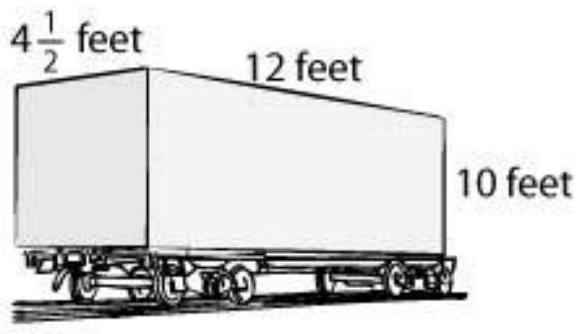
\includegraphics[width=0.88\linewidth]{math-6th/images/25b2bbb6-511f-4540-805d-d84ad3778da8-2_334_581_1443_1426}
  \end{center}
  \begin{solutionorbox}[0.9in]
  For $\frac{1}{2}$ inch cubes, divide each edge length by $\frac{1}{2}$ (double each dimension) and multiply the counts, or divide total volume by $\left(\frac{1}{2}\right)^3$.
  \end{solutionorbox}
\end{parts}

\question[5]
Which expressions are equivalent to $4(3e+8j)$? \emph{Select all that apply.}
\begin{checkboxes}
  \choice $12e+8j$
  \CorrectChoice $12e+32j$
  \choice $44ej$
  \CorrectChoice $11e+e+31j+j$
\end{checkboxes}
\begin{solution}
  $4(3e+8j)=12e+32j$; also $11e+e+31j+j=12e+32j$.
\end{solution}

\question[5]
Connor purchases a new car every $6$ years. Carolyn purchases a new car every $8$ years. They both purchased new cars this year. When will they next both purchase new cars in the same year?
\rightfillin{$24$ years from now}
\begin{solution}
  $\operatorname{lcm}(6,8)=24$.
\end{solution}

\question[5]
Simplify: $\left(\dfrac{4}{5}\right)^{4}$.
\begin{choices}
  \choice $\dfrac{16}{25}$
  \choice $\dfrac{64}{125}$
  \CorrectChoice $\dfrac{256}{625}$
  \choice $\dfrac{1024}{3125}$
\end{choices}
\begin{solution}
  $\left(\frac{4}{5}\right)^{4}=\frac{256}{625}$.
\end{solution}

\question[5]
Yvette read a word problem that used the phrase ``ten less than the product of four and a number.'' Which expression represents this phrase?
\begin{choices}
  \choice $10-4n$
  \choice $10-(4+n)$
  \CorrectChoice $4n-10$
  \choice $(4+n)-10$
\end{choices}
\begin{solution}
  ``Product of four and a number'' is $4n$; ten less is $4n-10$.
\end{solution}

\question[5]
A plumber charges customers $\$45$ for a service call plus $\$60$ per hour of repair. The expression $45+60h$ can be used to determine the total dollar amount of charges based on $h$ hours of repair. How much would it cost if the repair took $5$ hours?
\rightfillin{$\$345$}
\begin{solution}
  $45+60(5)=345$.
\end{solution}

\question[5]
Kiara baked $30$ oatmeal cookies and $48$ chocolate chip cookies to package in plastic containers for her friends at school. She wants to divide the cookies into identical containers so that each container has the same number of each kind of cookie. If she wants each container to have the greatest number of cookies possible, how many plastic containers does she need?
\begin{choices}
  \choice $3$
  \choice $4$
  \choice $5$
  \CorrectChoice $6$
\end{choices}
\begin{solution}
  $\gcd(30,48)=6$ containers (each with $5$ oatmeal and $8$ chocolate chip).
\end{solution}

\question[5]
A baker made a batch of cupcakes. He put $2$ candies on top of each cupcake. He used $48$ candies in all. Let $c$ represent the number of cupcakes in the batch. Which equation represents this?
\begin{choices}
  \choice $2+c=48$
  \choice $2-c=48$
  \choice $2\div c=48$
  \CorrectChoice $2c=48$
\end{choices}
\begin{solution}
  Two candies per cupcake: $2c=48$.
\end{solution}

\newpage

\question[5]
Consider this inequality: $z>-9$. Determine whether each value of $z$ makes this inequality true. Write \textbf{Yes} or \textbf{No}.
\labeledfillin{$z=-7$}{Yes}
\labeledfillin{$z=-4$}{Yes}
\labeledfillin{$z=0$}{Yes}
\begin{solution}
  Each listed value is greater than $-9$.
\end{solution}

\question[5]
Tia wants to get an $A$ in her math class. To earn an $A$ in the course, she must earn a mean score of at least $90$ on her $4$ exams. Which inequality represents this (using the same variable $e$ for each exam score, as in the original problem)?
\begin{choices}
  \choice $e>90$
  \choice $e<90$
  \CorrectChoice $e\ge 90$
  \choice $e\le 90$
\end{choices}
\begin{solution}
  If all four scores equal $e$, the mean is $e$, so requiring a mean of at least $90$ matches $e\ge 90$ in this template.
\end{solution}

\question[5]
Which of the following equations have the solution $x=3$? \emph{Select all that apply.}
\begin{checkboxes}
  \choice $\dfrac{x}{3}=9$
  \CorrectChoice $15x=45$
  \choice $\dfrac{1}{5}x=15$
  \CorrectChoice $12+x=15$
\end{checkboxes}
\begin{solution}
  For $x=3$: $15(3)=45$ and $12+3=15$. The other two equations are not satisfied when $x=3$.
\end{solution}

\question[10]
Which number line represents the inequality $m>350$?
\begin{choices}
  \choice
  \begin{minipage}[t]{0.82\linewidth}
    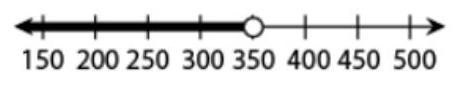
\includegraphics[width=\linewidth]{math-6th/images/25b2bbb6-511f-4540-805d-d84ad3778da8-4_85_459_1009_459}
  \end{minipage}
  \choice
  \begin{minipage}[t]{0.82\linewidth}
    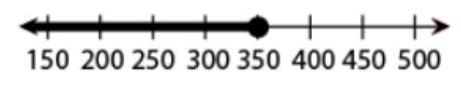
\includegraphics[width=\linewidth]{math-6th/images/25b2bbb6-511f-4540-805d-d84ad3778da8-4_85_461_1009_951}
  \end{minipage}
  \CorrectChoice
  \begin{minipage}[t]{0.82\linewidth}
    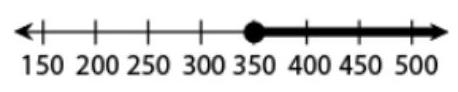
\includegraphics[width=\linewidth]{math-6th/images/25b2bbb6-511f-4540-805d-d84ad3778da8-4_92_458_1140_468}
  \end{minipage}
  \choice
  \begin{minipage}[t]{0.82\linewidth}
    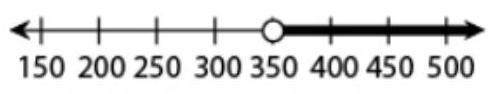
\includegraphics[width=\linewidth]{math-6th/images/25b2bbb6-511f-4540-805d-d84ad3778da8-4_94_497_1138_941}
  \end{minipage}
\end{choices}
\begin{solution}
  Choose the graph with an \emph{open} circle at $350$ and shading to the right (verify on your answer key image set).
\end{solution}

\question[5]
Reflect the following points.
\labeledfillin{$(1,-7)$ over the $x$-axis}{$(1,7)$}
\labeledfillin{$(-5,9)$ over the $y$-axis}{$(5,9)$}
\begin{solution}
  Reflect over $x$-axis: negate $y$; over $y$-axis: negate $x$.
\end{solution}

\question[5]
Find the distance between the following pairs of points.
\labeledfillin{$(-5,9)$ and $(-5,12)$}{$3$}
\labeledfillin{$(-2,-9)$ and $(5,-9)$}{$7$}
\begin{solution}
  Same $x$: distance $|12-9|=3$. Same $y$: distance $|5-(-2)|=7$.
\end{solution}

\question[10]
What is the area of the triangle?
\begin{center}
  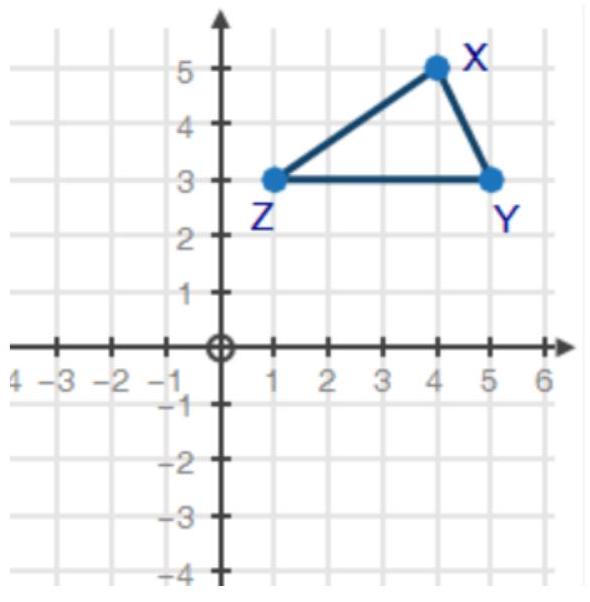
\includegraphics[width=0.88\linewidth]{math-6th/images/25b2bbb6-511f-4540-805d-d84ad3778da8-4_602_590_2015_758}
\end{center}
\begin{solutionorbox}[1.2in]
  Use $A=\dfrac{1}{2}bh$ with base and height read from the diagram.
\end{solutionorbox}

\endgradingrange{allmilestones}
